% siminos/spatiotemp/chapter/prime.tex  % called by blogCats.tex and CL18.tex
% $Author: predrag $ $Date: 2021-08-10 11:56:19 -0400 (Tue, 10 Aug 2021) $

\section{Enumeration of prime \twots}
\label{sect:Count2dprimePO}

\begin{description}

    \PCpost{2020-08-10}{
Copied to  \emph{siminos/kittens/prime.tex}, in  \emph{CL18.tex}
The two versions are from now on edited separately
	}

\end{description}


\subsection{Covering alphabet}
\label{sect:prime2tCover}

Our algorithm for generating all prime $\LTS{}{}{}$ Bravais
lattices consists in picking the lexically lowest \brick\
for every set of \brick s related by spatial and temporal translations:
\begin{enumerate}
  \item
Fill the first row
\(
\left[\Ssym{11}\;\Ssym{21}\cdots\Ssym{\speriod{}1}\right]
\)
by lexically ordered symbols,
\(
\Ssym{j1}\leq\Ssym{j+1,1}\,,
\)
keep one \brick\ for each set of spatially cyclically related
permutations.
  \item
Picking the lexically ordered first row representatives uses up the
cyclic invariance under spatial translations, so for the second
\(
\left[\Ssym{12}\;\Ssym{22}\cdots\Ssym{\speriod{}2}\right]
\)
and higher rows fill in all $|\A|^\period{}$ combinations of  symbols.
  \item
The count is the same for all $\LTS{}{}{}$
relative-periodic {\brick}s.
  \item
Group \brick s into sets related by cyclic permutations in the time
direction. For each such set, pick a representative that has lexically
lowest first row, throw away the rest.
  \item
Throw away all {\brick}s which are repeats of
shorter {\brick}s in the spatial direction.
  \item
Throw away all {\brick}s which are repeats of
shorter {\brick}s in the temporal direction. What
remains in $N_k$ prime periodic \brick s $p$ of the same size
$[\speriod{p}\times\period{p}]=[\speriod{k}\times\period{k}]$.
  \item
The total number
of (doubly) periodic
\brick s is the sum of all cyclic permutations of prime \brick s,
\[
|\A|^{\speriod{}\period{}}
=
\sum_p N_{p}\,\LTS{p}{p}{p}
\]
where the sum goes over prime tilings of the $\LTS{}{}{}$
\brick.
\end{enumerate}
This completes the list of prime \twots, with the alphabet $\A$ taken
as a {\em covering} alphabet, \ie, we have generated all possible prime
\brick s, under assumption of no grammar rules.

\PCedit{
The number of prime \twots\ is given recursively by
(see \refeq{primeCount}),
\beq
M_{p}\,=\,\frac{1}{\speriod{}\period{}}
  \left( N_{p}
          - \sum _{p'}
            \speriod{p'}\period{p'}
                                          \, M_{p'}
  \right)
\,,
\ee{primeCount2D}
where the sum is over $p'$, the prime `divisors' of $p$
that satisfy tiling conditions \refeq{primeTiling}.
    }

\bigskip

\noindent{\em Example: $\BravCell{2}{2}{0}$ Bravais
                lattices prime {\brick}s.}
%\label{sect:prime2tori2x2}

%    \HLpost{2019-11-22}{
Consider $\BravCell{2}{2}{0}$ Bravais
lattices prime {\brick}
\beq
\Mm_p=
        \left[\begin{array}{cc}
\Ssym{01} & \Ssym{11}   \\
\Ssym{00} & \Ssym{10}
              \end{array}\right]
\,,
\ee{eq:block2x2}
and the relative-periodic $\BravCell{2}{1}{1}$ {\brick} with $1$ site-shift
periodic boundary, which is periodic after the second repeat in the time
direction,
\beq
\Mm_p=
        \left[\begin{array}{ccc}
           &  \left[\Ssym{00}\right.&\left.\Ssym{10}\right] \\
\left[\Ssym{00}\right.&\left.\Ssym{10}\right] &
         \end{array}\right]
\,.
\ee{eq:block2x1rp}
According to \refeq{primeCount2D}, the number of prime % primitive
$\BravCell{2}{2}{0}$ {\lattstate}s is
\bea
M_{\BravCell{2}{2}{0}}&=&\frac{1}{2\cdot2}
  \left( N_{\BravCell{2}{2}{0}}
            - 2M_{\BravCell{2}{1}{0}}
%    \right.\ceq\left.\qquad\qquad
            - 2M_{\BravCell{1}{2}{0}}
            - 2M_{\BravCell{2}{1}{1}}
            - M_{\BravCell{1}{1}{0}}
  \right)
\,,
\label{catlattM2x2}
\eea
We can work this out explicitly as follows:\\
(1)
Fill the first row
\(
\left[\Ssym{11}\;\Ssym{21}\right]
\)
by lexically ordered symbols, one for each set of spatially cyclically related
permutations. For the alphabet \refeq{catLatt2d} there
are 36
such length 2 strings.

(2) As we have already `used up' the cyclic invariance under spatial
translations by picking the lexically ordered first row representatives,
for the second
\(
\left[\Ssym{12}\;\Ssym{22}\right]
\)
and higher rows all 81 combinations of 9 symbols are allowed.
We now have $36\times81 =2916$ {\brick}s in all.

(3) The $\BravCell{2}{1}{1}$ relative-periodic {\brick} \refeq{eq:block2x1rp} is
counted as the $\BravCell{2}{2}{0}$ \twot; as in (1), after spatial cyclic
rotations, there are 36 such prime {\brick}s.

(4) Group \brick s into sets related by cyclic permutations in the time
direction. For each such set, pick a representative that is lexically
lowest in the first row, throw away the rest.

(5) Throw away all {\brick}s which are repeats of
shorter {\brick}s. There are three kinds of repeating small {\brick}s:
\[
\BravCell{2}{1}{0}=\left[\begin{array}{cc}
a & b \\
a & b \\
              \end{array}\right]
\, , \quad
\BravCell{1}{2}{0}=\left[\begin{array}{cc}
b & b \\
a & a \\
              \end{array}\right]
\, , \quad
\BravCell{2}{1}{1}=\left[\begin{array}{ccc}
  & a & b \\
a & b &   \\
              \end{array}\right]
\,.
\]
(6)
The result is 1584 $\BravCell{2}{2}{0}$ prime {\brick}s.

There are also 36 prime $\BravCell{2}{1}{0}$ {\brick}s repeating in time, 36
prime $\BravCell{1}{2}{0}$ {\brick}s repeating in space, 36 prime $\BravCell{2}{1}{1}$
{\brick}s repeating in time with $1/2$-shift periodic boundary, and 9
{\brick}s which are repeats of one-symbol prime $\BravCell{1}{1}{0}$ {\brick}.
The total number
of \PCedit{$\BravCell{2}{2}{0}$} % 2019-11-22 Han's was $[4\times4]$
\brick s is recovered by all cyclic permutations of prime \brick s \refeq{catlattM2x2}:
\bea
N_{\BravCell{2}{2}{0}} &=& 9^{2\times2} = 6561
    \label{catlattN2x2}\\
    &=&        {1584}\,\BravCell{2}{2}{0}
             + {36}\,\BravCell{2}{1}{0}
             + {36}\,\BravCell{1}{2}{0}
             + {36}\,\BravCell{2}{1}{1}
             + {9}\,\BravCell{1}{1}{0}
\,,
\nnu
\eea
where $\cycle{\cdots}$ stands for the number of prime {\brick}s
of a given shape.
This completes the count with the alphabet
\refeq{catLatt2d} taken as a {\em covering} alphabet, \ie, we
have generated all possible prime \brick s, were there no further grammar
rules.

\bigskip

\noindent{\em Example: $\BravCell{3}{2}{0}$  Bravais
                lattices prime {\brick}s.}
%\label{sect:prime2tori3x2}

Consider the Bravais lattice
\beq
\Mm=
        \left[\begin{array}{ccc}
\Ssym{12} & \Ssym{22} & \Ssym{32}   \\
\Ssym{11} & \Ssym{21} & \Ssym{31}
              \end{array}\right]
\,.
\ee{eq:block3x2}
According to \refeq{primeCount2D}, the number of prime %primitive
$\BravCell{3}{2}{0}$ {\lattstate}s is
\bea
M_{\BravCell{3}{2}{0}}&=&\frac{1}{3\cdot2}
  \left( N_{\BravCell{3}{2}{0}}
            - 3M_{\BravCell{3}{1}{0}}
%    \right.\ceq\left.\qquad\qquad
            - 2M_{\BravCell{1}{2}{0}}
            - M_{\BravCell{1}{1}{0}}
  \right)
\,,
\label{catlattM3x2}
\eea
Unlike the $\BravCell{2}{2}{0}$ case \refeq{eq:block2x1rp}, there no sub-\brick s
with relative-periodic boundary contributing to the $\BravCell{3}{2}{0}$ \brick s
count, since $\BravCell{3}{1}{0}$ and $\BravCell{1}{2}{0}$ sub-\brick s cannot fit into
the $\BravCell{3}{2}{0}$ doubly-periodic Bravais lattice without a shift.

Following the same algorithm as for $\BravCell{2}{2}{0}$ \brick s, we get 88440
$\BravCell{3}{2}{0}$ prime \brick s, 240 prime $\BravCell{3}{1}{0}$ \brick
s repeating in time, 36 prime $\BravCell{1}{2}{0}$ \brick s repeating in space,
and 9 \brick s which are repeats of one symbol prime $\BravCell{1}{1}{0}$ \brick.
The total number of $\BravCell{3}{2}{0}$ \brick s is recovered by all cyclic
permutations of prime \brick s:
\bea
N_{\BravCell{3}{2}{0}} &=& 9^{3\times2} = 531441
    \continue
 &=& 88440\,\BravCell{3}{2}{0}+240\,\BravCell{3}{1}{0}
       +36\,\BravCell{1}{2}{0}+9\,\BravCell{1}{1}{0}
\,.
\label{catlattN3x2}
\eea



\subsection{Admissible prime \twots}
\label{sect:prime2tAdmiss}

To determine the {\em \admissible} \brick s, compute $\Xx_p$ for each
prime \brick\ $\Mm_p$, and eliminate every $\Xx_p$ which contains a
lattice site or sites on which the value of the field violates the
admissibility condition $\ssp_z\in[0,1)^2$.

%%%%%%%%%%%%%%%%%%%%%%%%%%%%%%%%%%%%%%%%%%%%%%%%%%%%%%
\ifblog
% siminos/spatiotemp/tables/LxTs5o2.tex
% $Author: predrag $ $Date: 2021-08-10 11:56:19 -0400 (Tue, 10 Aug 2021) $

%%%%%%%%%%%%%%%%%%%%%%%%%%%%%%%%%%%%%%%%%%%%%%%%%%%%%%
% called by blogCats.tex and CL18.tex
% 2020-06-09 HL siminos/mathematica/PrimeSolutions.nb
%            Edited the tables of numbers of prime solutions
% Predrag 2019-11-23 started with ChaosBook \reftab{tab:primeTwots}
\begin{table}
\caption[]{\label{tab:LxTs=5/2}    \small
The numbers of the ${s}=5/2$ \catlatt\
$\LTS{}{}{}$ \twots: $M_{\LTS{}{}{}}$ is the
number of prime \twots, $N_{\LTS{}{}{}}$ is the
number of doubly periodic {\lattstate}s,
and $R_{\LTS{}{}{}}$ is the number of prime \twots\ in the
$\Dn{4}$ symmetries orbit.
}
\begin{center}
%\renewcommand{\arraystretch}{0.8}
{\small
\begin{tabular}{lrlr}
\\[-16pt]
$\LTS{}{}{}$
                  & $M$ %_{[\speriod{}\!\times\!\period{}]}$
                         & $N$ %_{[\speriod{}\!\times\!\period{}]}$
                                                 &$R$\\
\hline
$\BravCell{1}{1}{0}$  &   1  &   1                   & 1 \\
$\BravCell{2}{1}{0}$  &   2  &
  $5~=\;\;\,2\,\BravCell{2}{1}{0}+1\,\BravCell{1}{1}{0}$
                                                 & 2 \\
$\BravCell{2}{1}{1}$&   4  & 9~\;=\;\;\,$
                           {4}\,\BravCell{2}{1}{1}
                         + {1}\,\BravCell{1}{1}{0}$
                                                 &   \\
$\BravCell{3}{1}{0}$  &   5  & 16 =~ ${5}\,\BravCell{3}{1}{0}
                         + {1}\,\BravCell{1}{1}{0}$
                                                 &   \\
$\BravCell{3}{1}{1}$&   16 & $49 =16\,\BravCell{3}{1}{1}
                         + {1}\,\BravCell{1}{1}{0}$
                                                 &   \\
%$\BravCell{3}{1}{2}$&   16 & $49 =16\,\BravCell{3}{1}{2}  % (49-1)/3
%                         + {1}\,\BravCell{1}{1}{0}$
%                                                 &   \\
$\BravCell{4}{1}{0}$  &  10 & $45 =10\,\BravCell{4}{1}{0} % (45-2*2-1)/4
                         + {2}\,\BravCell{2}{1}{0}
                         + {1}\,\BravCell{1}{1}{0}$
                                                 &   \\
$\BravCell{4}{1}{1}$&   54 & $225 =54\,\BravCell{4}{1}{1} % (225-4*2-1)/4
			+{4}\,\BravCell{2}{1}{1}
                         + {1}\,\BravCell{1}{1}{0}$
                                                 &   \\
$\BravCell{4}{1}{2}$&   60 & $245 =59\,\BravCell{4}{1}{2} % (245-2*2-1)/4
                         + {2}\,\BravCell{2}{1}{0}
                         + {1}\,\BravCell{1}{1}{0}$
                                                 &   \\
%$\BravCell{4}{1}{3}$&   56 & $225 =56\,\BravCell{4}{1}{2}
%                         + {1}\,\BravCell{1}{1}{0}$
%                                                 &   \\
$\BravCell{2}{2}{0}$  &   52  & $225 =
               {52}\,\BravCell{2}{2}{0}
             + {2}\,\BravCell{2}{1}{0}
             + {2}\,\BravCell{1}{2}{0}$
                                                 &   \\
                      &       & $\quad\quad\;\;
             + {4}\,\BravCell{2}{1}{1}
             + {1}\,\BravCell{1}{1}{0}$
                                                 & 1 \\
$\BravCell{2}{2}{1}$&  60 & $245 = 60\,\BravCell{2}{2}{1}  % (245-2*2-1)/4
			+ {2}\,\BravCell{1}{2}{0}
                         + {1}\,\BravCell{1}{1}{0}$
                                                 &   \\
$\BravCell{3}{2}{0}$  & 850  &
                          $ 5\,120 =850\,\BravCell{3}{2}{0}
                          +5\,\BravCell{3}{1}{0}$
                                                 &   \\
                      &       & $\qquad\quad\;\,
                          +2\,\BravCell{1}{2}{0}
                          +1\,\BravCell{1}{1}{0}$
                                                 &   \\
$\BravCell{3}{2}{1}$& 1\,012 &
                           $ 6\,125 =1\,012\,\BravCell{3}{2}{1} %(6125 - 16*3-2*2 -1)/6
                           +16\,\BravCell{3}{1}{2}$
                                                 &   \\
                      &       & $\qquad\quad~~
                           +2\,\BravCell{1}{2}{0}
                           +~\,1\,\BravCell{1}{1}{0}$
                                                 &   \\
%$\BravCell{3}{2}{2}$&      & 6125 =?$\BravCell{3}{2}{2}
%                         + {1}\,\BravCell{1}{1}{0}$
%                                                 &   \\
$\BravCell{3}{3}{0}$  & 68\,281 &

                         $ 614\,656 = 68\,281\,\BravCell{3}{3}{0}
                         +  5\,\BravCell{3}{1}{0}$  %(614656 -2*16*3 - 5*3 - 5*3 -1)/9$
                                                 &   \\
                      &       & $\,
                         + 16\,\BravCell{3}{1}{1} +16 \,\BravCell{3}{1}{2}
                         +  5\,\BravCell{1}{3}{0}
                         + {1}\,\BravCell{1}{1}{0}$
                                                 & 1  \\
$\BravCell{3}{3}{1}$& 70\,400  &
                         $ 633\,616 =70\,400\,\BravCell{3}{3}{1}
                         + {5}\,\BravCell{1}{3}{0} %(633616 - 5*3 -1)/9
                         + {1}\,\BravCell{1}{1}{0}$
                                                 &   \\
%$\BravCell{3}{3}{2}$&      & 633616 =?$\BravCell{3}{3}{2}
%                         + {1}\,\BravCell{1}{1}{0}$
%                                                 &   \\
\end{tabular}
} %end \small
\end{center}
\end{table}
%%%%%%%%%%%%%%%%%%%%%%%%%%%%%%%%%%%%%%%%%%%%%%%%%%%%%%%%%%%%%%%%%%%%%%

\fi
%%%%%%%%%%%%%%%%%%%%%%%%%%%%%%%%%%%%%%%%%%%%%%%%%%%%%%


\begin{description}

    \HLpost{2019-11-22}{
For $s=5/2$ \catlatt\ the pruning is very severe. Of {1584}
covering alphabet prime {\brick}s in \refeq{catlattN2x2}, only 52 prime
\PCedit{$\BravCell{2}{2}{0}$} % 2019-11-22 Han's was $[4\times4]$
{\brick}s are {\admissible}. As for the repeats of smaller {\brick}s,
there are 2 {\admissible} $\BravCell{1}{2}{0}$ {\brick}s repeating in time and 2
$\BravCell{2}{1}{0}$ {\brick}s repeating in space. There are 4 {\admissible}
$1/2$-shift periodic boundary $\BravCell{1}{2}{0}$ {\brick}s. And there is 1
admissible {\brick} $\BravCell{1}{1}{0}$ which is a repeat of letter 0.
The total number of $\BravCell{2}{2}{0}$ of \twots\ is obtained by all cyclic
permutations of \admissible\ prime \brick s (a significant pruning,
compared to the full shift count \refeq{catlattN2x2}),
\bea
N_{\BravCell{2}{2}{0}} &=& 225
 \label{HL[2x2]count}\\
    &=&       {52}\,\BravCell{2}{2}{0}
             + {2}\,\BravCell{2}{1}{0}
             + {2}\,\BravCell{1}{2}{0}
             + {4}\,\BravCell{2}{1}{1}
             + {1}\,\BravCell{1}{1}{0}
\,.
\nnu
\eea
    }

    \HLpost{2019-11-23}{
For $s=5/2$ \catlatt\
only 850 prime $\BravCell{3}{2}{0}$ \brick s are \admissible. There are 5
\admissible\ repeating prime $\BravCell{3}{1}{0}$ \brick s, 2 \admissible\
repeating prime $\BravCell{1}{2}{0}$ \brick s, and 1 \admissible\ \brick\ which
is a repeat of 0. The total number of \admissible\ solutions obtained by
all cyclic permutations of \admissible\ prime \brick s is:
     \beq
N_{\BravCell{3}{2}{0}} = 5120
=850\,\BravCell{3}{2}{0}+5\,\BravCell{3}{1}{0}+2\,\BravCell{1}{2}{0}+1\,\BravCell{1}{1}{0}
\,,
     \ee{HL[3x2]count}
in agreement with the counting formula \refeq{2DCountingFormula}
for the $\BravCell{3}{2}{0}$ \twots.
    }

%%%%%%%%%%%%%%%%%%%%%%%%%%%%%%%%%%%%%%%%%%%%%%%%%%%%%%
\ifblog
% siminos/spatiotemp/tables/LxTs.tex
% $Author: predrag $ $Date: 2021-08-10 11:56:19 -0400 (Tue, 10 Aug 2021) $

%%%%%%%%%%%%%%%%%%%%%%%%%%%%%%%%%%%%%%%%%%%%%%%%%%%%%%
% 2020-06-09 HL siminos/mathematica/PrimeSolutions.nb
%            Edited the tables of numbers of prime solutions
% Predrag 2020-02-23    called by blogCats.tex and CL18.tex
\begin{table}
\caption[]{\label{tab:LxTs}     \small
The numbers of \catlatt\ {\lattstate}s for Bravais lattices
$\Lambda=\LTS{}{}{}$ up to $\BravCell{3}{3}{2}$. Here
$N_\Lambda(s)$ is the number of doubly periodic
{\lattstate}s,
$M_\Lambda(s)$ is the number of prime \twots,
and $R_{\Lambda}$ is the number
of prime \twots\ in the $\Dn{4}$ symmetries orbit.
The stretching parameter ${s}$ can take half-integer or integer
values.
}
\begin{center}
%\renewcommand{\arraystretch}{0.8}
{\small
\begin{tabular}{lllr}
\\[-16pt]
$~~~\Lambda$
                         & ~~~$N_\Lambda(s)$ & $M_\Lambda(s)$
                                                 &$R$  \\
\hline
$\BravCell{1}{1}{0}$    &   $2({s}-2)$ & $2({s}-2)$ & 1 \\
$\BravCell{2}{1}{0}$    &   $2({s}-2)2s$ & $2({s}-2)\frac{1}{2}(2{s}-1)$   & 2 \\
$\BravCell{2}{1}{1}$  &   $2({s}-2)2({s}+2)$ & $2({s}-2)\frac{1}{2}(2{s}+3)$  & \\
$\BravCell{3}{1}{0}$    &   $2({s}-2)(2{s}-1)^2$ & $2({s}-2)\frac{4}{3}({s}-1){s}$ &  \\
$\BravCell{3}{1}{1}$  &   $2({s}-2)4({s}+1)^2$ & $2({s}-2)\frac{1}{3}(2{s}+1)(2{s}+3)$ & \\
%was $2({s}-2)(2{s}-1)^2$
%$\BravCell{3}{1}{2}$  &   $2({s}-2)4({s}+1)^2$ & $2({s}-2)\frac{1}{3}(2{s}+1)(2{s}+3)$ & \\
%was $2({s}-2)(2{s}-1)^2$
$\BravCell{4}{1}{0}$    &   $2({s}-2)8({s}-1)^2{s}$ & $2({s}-2)\frac{1}{2}(2{s}-3)(2{s}-1)s$ & \\
$\BravCell{4}{1}{1}$  &   $2({s}-2)8s^2({s}+2)$ & $2({s}-2)\frac{1}{2}({s}+2)(2{s}-1)(2{s}+1)$ & \\
%was $2({s}-2)8({s}-1)^2{s}$
$\BravCell{4}{1}{2}$  &   $2({s}-2)8({s}+1)^2{s}$ & $2({s}-2)\frac{1}{2}(2{s}+3)(2{s}+1)s$     & \\
%was $2({s}-2)8({s}-1)^2{s}$
$\BravCell{4}{1}{3}$  &   $2({s}-2)8s^2({s}+2)$ & $2({s}-2)\frac{1}{2}({s}+2)(2{s}-1)(2{s}+1)$ &  \\
%was $2({s}-2)8({s}-1)^2{s}$
$\BravCell{5}{1}{0}$    & $2({s}-2)\left(4{s}^2-6{s}+1\right)^2$ & $2({s}-2)\frac{4}{5}({s}-1)(2{s}-3)(2{s}-1)s$
                                  & \\
$\BravCell{5}{1}{1}$  & $2({s}-2)16\left({s}^2+{s}-1\right)^2$ & $2({s}-2)\frac{1}{5}(2{s}-1)(2{s}+3)(4{s}^2+4{s}-5)$
                                  & \\
%was $2({s}-2)\left(4{s}^2-6{s}+1\right)^2$
$\BravCell{2}{2}{0}$    & $2({s}-2)8s^2({s}+2)$ & $2({s}-2)\frac{1}{2}(2{s}-1)(2{s}^2+5{s}+1)$  & 1 \\
$\BravCell{2}{2}{1}$  & $2(s-2)8s (s+1)^2$ & $2({s}-2)\frac{1}{2}(2{s}+1)(2{s}+3)s$ &  \\
%was $2(s-2)8s^2 (s+2)$
$\BravCell{3}{2}{0}$    & $2({s}-2)2s(2{s}-1)^2 (2{s}+3)^2$
	& $2({s}-2)\frac{2}{3}(2{s}-1)(4{s}^3+10{s}^2+3{s}-5)s$
                                  &  \\
$\BravCell{3}{2}{1}$  & $2({s}-2)32{s}^3({s}+1)^2$
	& $2 ({s}-2) \frac{1}{6} (2 {s}-1) (2 {s}+1) (8 {s}^3+16 {s}^2+10 {s}+3)$
                                  &  \\
%$\BravCell{3}{2}{2}$  & $2({s}-2)32{s}^3 ({s}+1)^2$
%	& $2 ({s}-2) \frac{1}{6} (2 {s}-1) (2 {s}+1) (8 {s}^3+16 {s}^2+10 {s}+3)$
%                                  &  \\
$\BravCell{3}{3}{0}$    & $2({s}-2)16({s}+1)^4(2{s}-1)^4$
                                  &  \\
$\BravCell{3}{3}{1}$  & $2({s}-2)(2{s}-1)^2(8{s}^3+12{s}^2-1)^2$
	            &  \\
%$\BravCell{3}{3}{2}$  & $2({s}-2)(2{s}-1)^2(8{s}^3+12{s}^2-1)^2$
%                &
\end{tabular}
} %end \small
\end{center}
\end{table}
%%%%%%%%%%%%%%%%%%%%%%%%%%%%%%%%%%%%%%%%%%%%%%%%%%%%%%%%%%%%%%%%%%%%%%

\fi
%%%%%%%%%%%%%%%%%%%%%%%%%%%%%%%%%%%%%%%%%%%%%%%%%%%%%%%%%%%%%%%%%%%%%%

    \HLpost{2020-06-09}{
The \admissible\ prime \twots\ counts for any half-integer or integer
${s}$ are listed in \reftab{tab:LxTs}.
Note that $N_{\BravCell{3}{\period{}}{1}}({s})=N_{\BravCell{3}{\period{}}{2}}({s})$,
by reflection symmetry, as
$N_{\BravCell{3}{\period{}}{2}}({s})=N_{\BravCell{3}{\period{}}{-1}}({s})$.


These two expressions do not
fit into the table format:
\bea
M_{\BravCell{3}{3}{0}}
&=&
2({s}-2)\frac{1}{9}(256 {s}^8+512 {s}^7-128 {s}^6-640 {s}^5
\ceq
\qquad\quad +16 {s}^4+320 {s}^3-48 {s}^2-72 {s}+9)
\,.
\label{HL[3x3]0cnt}
\eea
The last, currently unreduced formula exemplifies what is nonintuitive
about the Fourier space results; it is not at all obvious that this
\bea
M_{\BravCell{3}{3}{1}}
&=&
M_{\BravCell{3}{3}{2}}
=
2 (s-2) \frac{1}{9} (1-2 s)^2 \times
\ceq
\left\{\left[2 s+1-2 \sin \left(\frac{\pi}{18}\right)\right]^2
\left[2 s+1+2 \cos \left(\frac{\pi}{9}\right)\right]^2
     \right.
\ceq
     \left.
~~\left[(2 s+1-2 \cos \left(\frac{2\pi}{9}\right)\right]^2-1
     \right\}
\label{HL[3x3]0count}
\eea
is an
integer for any half-integer or integer ${s}$.
{\bf Predrag} to Han: can you evaluate this using the fundamental fact
$N_\cl{} = |\Det\jMorb|$?
    }

    \HLpost{2020-06-09}{
The \admissible\ prime \twots\ counts are listed in
\reftab{tab:LxTs=5/2}. This list verifies the counting formula
\refeq{2DCountingFormula}.
    }

    \HLpost{2019-11-24}{
The interior alphabet depends on the value of $s$ and the \admissible\
range of $\ssp_z$.
For $s=5/2$, $\ssp_z\in[0,1)$, the interior alphabet is
$\Ai=\{0,1\}$ (see eq.~(38) in \refref{GHJSC16}).
For $s=7/2$, $\ssp_z\in[0,1)$, the interior alphabet is
$\Ai=\{0,1,2,3\}$ (eq.~(46) in \refref{GHJSC16}).
    }

	\HLpost{2020-06-09}{
\refFigs{fig:SpecialBravaisLatt}{fig:3x2rpo} are the plots of the
periodic \brick s by color. The three figures in
\reffig{fig:SpecialBravaisLatt} are the \brick s with periodicity
$\BravCell{1}{3}{0}$, $\BravCell{3}{1}{0}$ and $\BravCell{3}{1}{1}$,
which can show the periodicity of the space-\eqva, time-\eqva\ and
time-\reqva. \refFig{fig:3x2rpo} is the color coding of the periodic
blocks with periodicity $\BravCell{2}{1}{1}$, $\BravCell{3}{2}{1}$ and
$\BravCell{3}{2}{0}$.
	}

%%%%%%%%%%%%%%%%%%%%%%%%%%%%%%%%%%%%%%%%%%%%%%%%%%%%%%%%%%%%%
% HL 2020-06-09 siminos/figSrc/han/Mathematica/ColorBlock.nb
\begin{figure}\begin{center}
            \begin{minipage}[c]{0.25\textwidth}\begin{center}
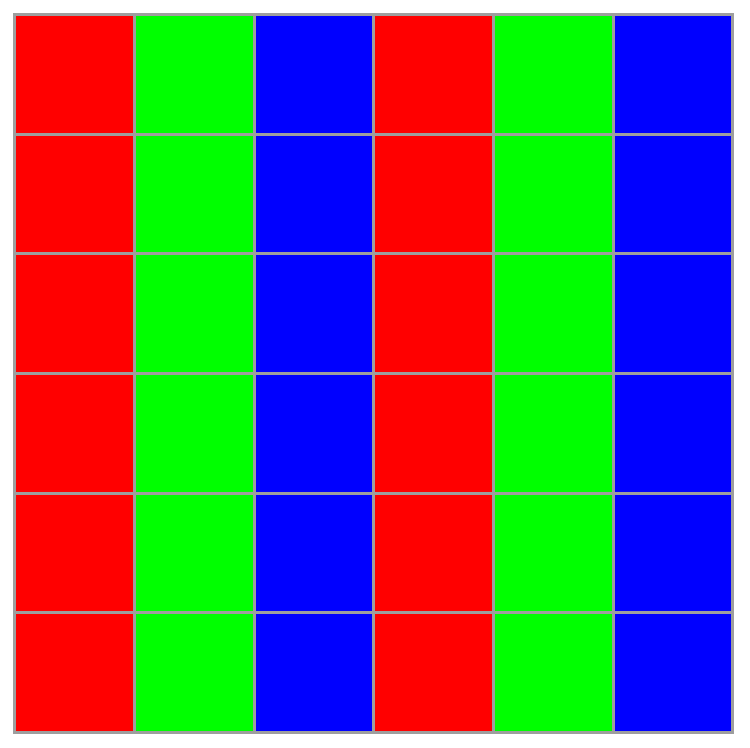
\includegraphics[width=1.0\textwidth]{HL310Block}\\(a)
            \end{center}\end{minipage}
            \hskip 4ex
            \begin{minipage}[c]{0.25\textwidth}\begin{center}
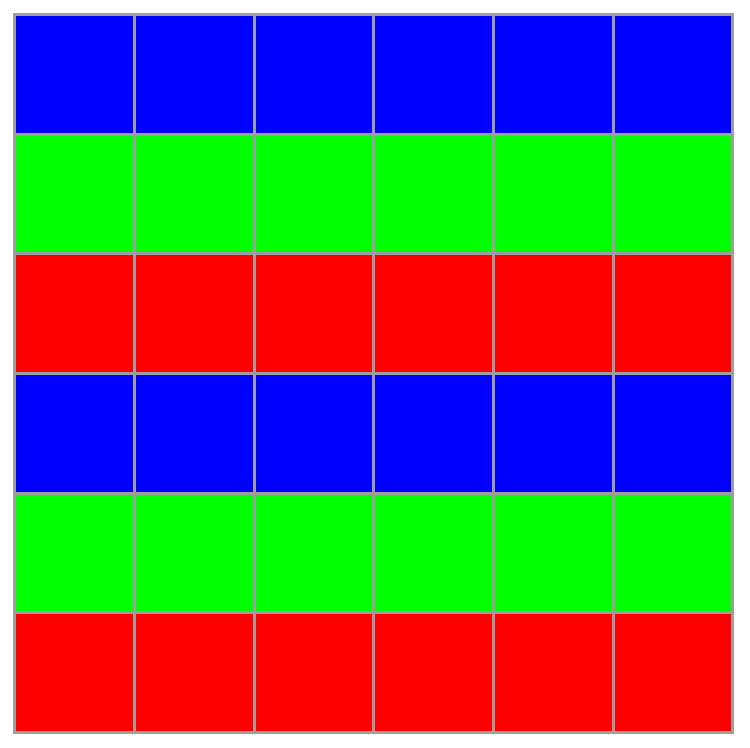
\includegraphics[width=1.0\textwidth]{HL130Block}\\(b)
            \end{center}\end{minipage}
            \hskip 4ex
            \begin{minipage}[c]{0.25\textwidth}\begin{center}
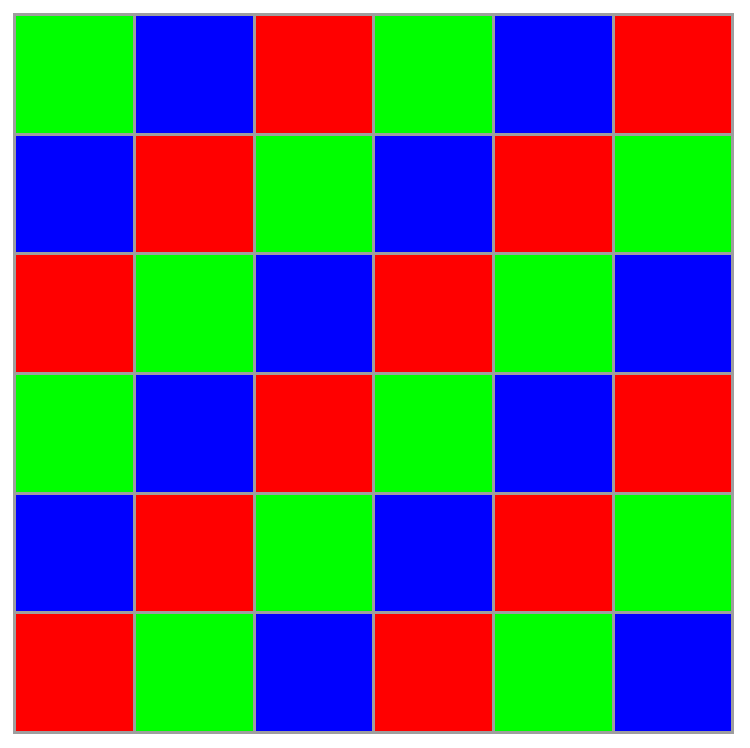
\includegraphics[width=1.0\textwidth]{HL311Block}\\(c)
            \end{center}\end{minipage}
\end{center}
  \caption{\label{fig:SpecialBravaisLatt}
Examples of $\LTS{}{}{}$ periodic \brick s
together with their \spt\ Bravais lattice tilings \refeq{2DBravaisLattice}.
(a)
$\BravCell{3}{1}{0}$, basis vectors
$\mathbf{a}_1=\{3,0\}$ and $\mathbf{a}_2=\{0,1\}$;
(b)
$\BravCell{1}{3}{0}$, basis vectors
$\mathbf{a}_1=\{1,0\}$ and $\mathbf{a}_2=\{0,3\}$;
(c)
$\BravCell{3}{1}{1}$, basis vectors
$\mathbf{a}_1=\{3,0\}$ and $\mathbf{a}_2=\{1,1\}$;
}
\end{figure}
%%%%%%%%%%%%%%%%%%%%%%%%%%%%%%%%%%%%%%%%%%%%%%%%%%%%%%%%%%%%%%%

%%%%%%%%%%%%%%%%%%%%%%%%%%%%%%%%%%%%%%%%%%%%%%%%%%%%%%%%%%%%%
% HL 2020-06-09 siminos/figSrc/han/Mathematica/ColorBlock.nb
\begin{figure}\begin{center}
            \begin{minipage}[c]{0.25\textwidth}\begin{center}
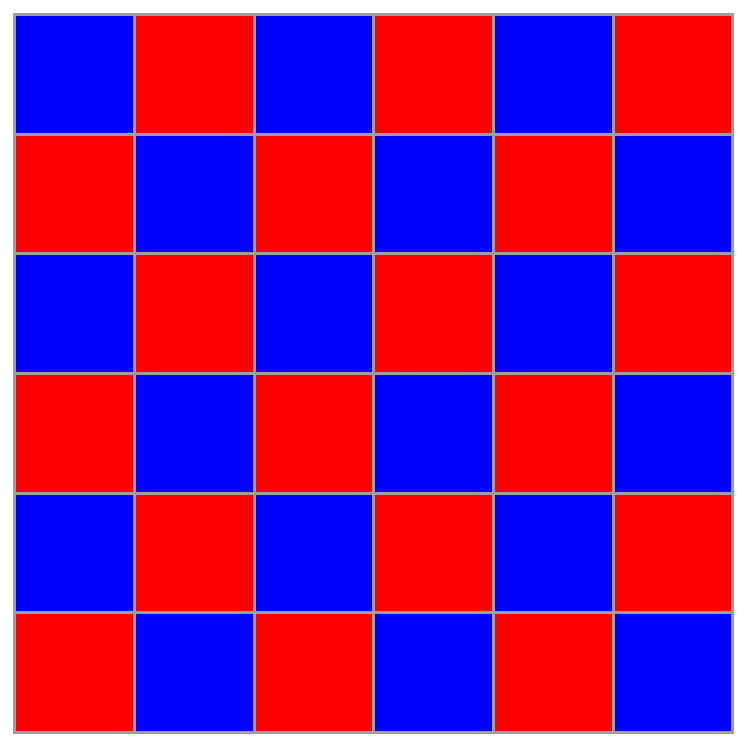
\includegraphics[width=1.0\textwidth]{HL211Block}\\(a)
            \end{center}\end{minipage}
            \hskip 4ex
            \begin{minipage}[c]{0.25\textwidth}\begin{center}
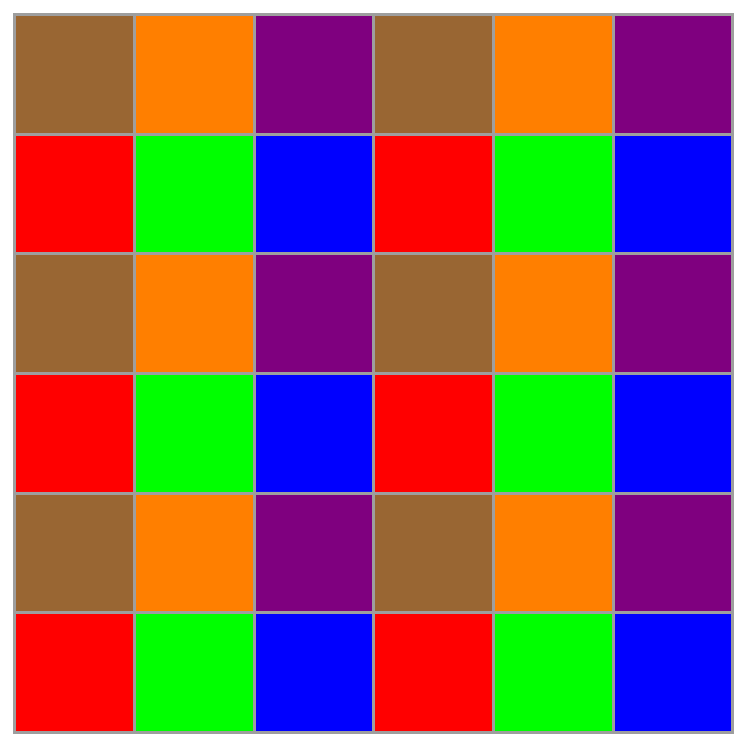
\includegraphics[width=1.0\textwidth]{HL320Block}\\(b)
            \end{center}\end{minipage}
            \hskip 4ex
            \begin{minipage}[c]{0.25\textwidth}\begin{center}
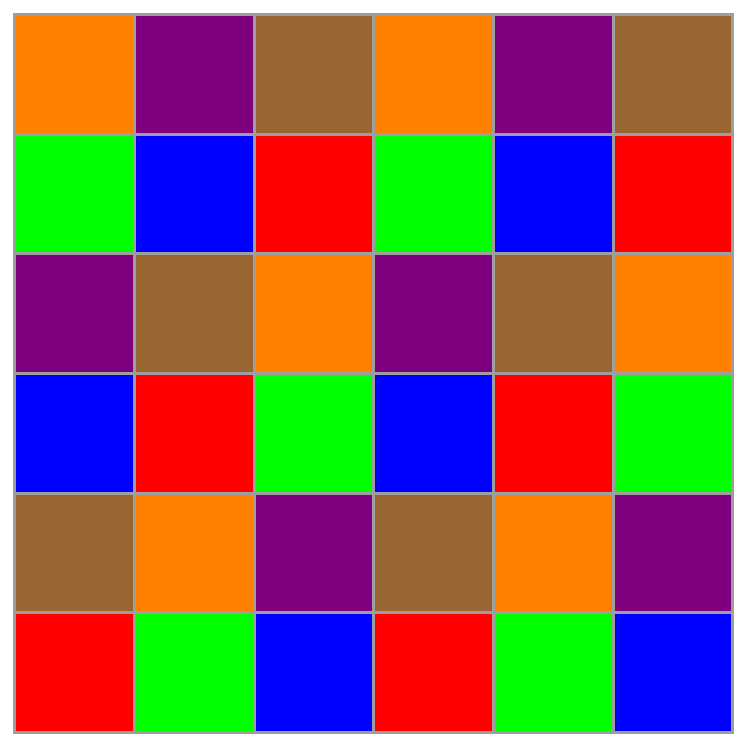
\includegraphics[width=1.0\textwidth]{HL321Block}\\(c)
            \end{center}\end{minipage}
\end{center}
  \caption{\label{fig:3x2rpo}
Examples of $\LTS{}{}{}$ periodic \brick s
together with their \spt\ Bravais lattice tilings \refeq{2DBravaisLattice}.
(a)
$\BravCell{2}{1}{1}$, basis vectors
$\mathbf{a}_1=\{2,0\}$ and $\mathbf{a}_2=\{1,1\}$;
(b)
$\BravCell{3}{2}{0}$, basis vectors
$\mathbf{a}_1=\{3,0\}$ and $\mathbf{a}_2=\{0,2\}$;
(c)
$\BravCell{3}{2}{1}$, basis vectors
$\mathbf{a}_1=\{3,0\}$ and $\mathbf{a}_2=\{1,2\}$;
}
\end{figure}
%%%%%%%%%%%%%%%%%%%%%%%%%%%%%%%%%%%%%%%%%%%%%%%%%%%%%%%%%%%%%%%



    \PCpost{2019-11-23}{
We always reduce relative-shift symmetries, so I am not happy about the
$\BravCell{2}{1}{1}$ relative-periodic {\brick} \refeq{eq:block2x1rp} being
counted as the $\BravCell{2}{2}{0}$ \twot. We'll have to revisit symmetry
reduction...
    }

    \PCpost{2019-11-23}{
For uses of the lexical ordering, ChaosBook table
\toChaosBook{section.18.2}
{18.1:} {\em {\Orbit}s for the binary symbolic dynamics up to length 9},
and appendix
\toChaosBook{section.R.2}
{A18.2} {\em Prime factorization for dynamical itineraries}
might be of interest.

In the paper, we will probably first review the \templatt\ counting,
something along the lines of the above tables.

suggestion of
constructing covering prime \brick s wildly overcounts the candidates for
\admissible\ prime \twots, so we should give up this avenue of
constructing them - no need to count any larger Bravais lattices.
    }


	\HLpost{2020-03-17}{
\emph{PrimeTiles.nb} generates all prime tiles that can tile a
larger tile. It gives
some not obvious results. For example, let the large tile be
$\BravCell{3}{2}{1}$, and consider the full-shift 9-symbol
$\BravCell{3}{2}{1}$ \brick s. The number $\BravCell{3}{2}{0}$ \brick s is
given by \refeq{catlattN3x2}. The program shows that the
$\BravCell{3}{2}{0}$ tile can only be tiled by $\BravCell{1}{1}{0}$,
$\BravCell{1}{2}{0}$ and $\BravCell{3}{1}{0}$ tiles. So we get the result in
\refeq{catlattN3x2}:
\[
N_{\BravCell{3}{2}{0}} = 9^{3\times2} =
88440\,\BravCell{3}{2}{0}+240\,\BravCell{3}{1}{0}
  +36\,\BravCell{1}{2}{0}+9\,\BravCell{1}{1}{0}
\,.
\]
For the full-shift the number of periodic \brick s is given
by the area of the larger tile, and number of $\BravCell{3}{2}{\tilt{}}$ \brick
s is the same for all $S$. But now
$\BravCell{3}{1}{0}$ tile cannot tile the $\BravCell{3}{2}{1}$ tile.
Instead, the $\BravCell{3}{2}{1}$ can be tiled by
$\BravCell{1}{1}{0}$, $\BravCell{3}{1}{2}$  and $\BravCell{1}{2}{0}$ tiles,
 \[
N_{\BravCell{3}{2}{1}} = 9^{3\times2} =
88440\,\BravCell{3}{2}{1}+ 240\,\BravCell{3}{1}{2}+36\,\BravCell{1}{2}{0}
   +9\,\BravCell{1}{1}{0}
\,.
\]
\emph{A priori} is not obvious that $\BravCell{3}{1}{2}$ tile can tile a
$\BravCell{3}{2}{1}$ tile. But if you stack $\BravCell{3}{1}{2}$ tile in the
shifted temporal direction by 2 then the left edge of the tile is shifted
by 4 in the spatial direction. With the spatial period being 3, shifted
by 4 in the spatial direction is same as shifted by 1. So the \bcs\ of
$\BravCell{3}{2}{1}$ tile are satisfied by the $\BravCell{3}{1}{2}$ tiles.
    }


\end{description}


%%%%%%%%%%%%%%%%%%%%%%%%%%%%%%%%%%%%%%%%%%%%%%%%%%%%%%%%%%%%%%%%%%%%%%%
%\printbibliography[heading=subbibintoc,title={References}]
